\documentclass[10pt,a4paper]{report}
\usepackage[utf8]{inputenc}
\usepackage{amsmath}
\usepackage{amsfonts}
\usepackage{amssymb}
\usepackage{graphicx}
\usepackage{fourier}
\newcommand{\abbrlabel}[1]{\makebox[3cm][l]{\textbf{#1}\ \dotfill}}
\newenvironment{abbreviations}{\begin{list}{}{\renewcommand{\makelabel}{\abbrlabel}}}{\end{list}}
\title{\begin{Large}
\textbf{Sensor Network For Pollution Monitoring}
\end{Large}\\ Master's Thesis Proposal}
\author{Ashlin Saju}

\date{}
\begin{document}

\maketitle
\tableofcontents
\newpage

\chapter{Introduction}Air pollution is a complex mixture of gases and particles whose sources and composition vary over space and time\cite{HealthEffectsInstitute2017}. The burning of fossil fuels, exhaust from factories and industries, and mining operations are the major contributors to air pollution. The major impacts of air pollution are premature deaths, cardiovascular disease, stroke, and other respiratory diseases. The state of global air 2017 has discussed the effects of long-term exposure to harmful air pollutants such as particulate matter which contributes to over 4 million premature deaths and is estimated to double by 2050 if the issue remains unattended\cite{HealthEffectsInstitute2017}. Therefore, the urgency for a global attention to mitigate the issue require no further emphasis. Among the risk factors with the serious health issues, Air pollution ranks the highest annually accounting for majority of deaths. Air pollution has increased significantly after the industrialization and urbanization have taken place, and people are unaware of the fact that the impact it causes to our health. As urban areas have a high density of population, maintaining air quality is becoming more and more challenging\cite{DCRMG17}.\\
					
					To address this epidemic issue, I believe, active participation from public on collecting and interpreting data, educating the behavior of individuals and industries, and helping to control and manage pollution sources effectively is crucial. Fortunately, this goal appears to be achievable due to the electronic and computing revolutions. It is possible that small, inexpensive, portable, and off-the-shelf pollution sensors along with low power processors and wireless communication modules can be bought at low cost. One of the important components in solving this issue is to increase the awareness among all stakeholders, particularly common people about the current situation and its impact so that they can act on it. The conventional method of monitoring the air quality with the help of a few heavyweight expensive stationary monitoring systems typically installed by the state may not be effective enough for this task. To achieve the goal effectively and without further delay, pollution monitoring must become part of daily activity for everyone. For that the devices to monitor pollution must be small, portable, inexpensive, and part of a global system.\\
 
  With the technological advancement of low cost computing, communication, and sensing devices, and the revolution and the importance of open source software\cite{A16}, I believe it is possible to build pervasive air pollution monitoring system with commodity hardware and open source software. Now the question is how to design such pollution monitoring devices faster and make them accessible to as many as possible.
Achieving the above stated goal requires a suitable system framework that can help to accelerate the process of the design and implementation of a air pollution monitoring system using the of-the-shelf commodity hardware and open source software. There are some recent attempts in this direction, but none is comprehensive and simple enough to follow and build a air pollution monitoring system with a little or moderate effort. 


\chapter{ Background and Related Work}
This chapter shows the major research work done on this field, it can be seen that most of the work are done on indoor pollution, since it is easy for evaluation.
\section{Development of Personal Integrated Environmental Monitoring System}

Pollution in urban areas are increasing rapidly and due to which the number of people suffering chronic illness, permanent disability or even death are also increasing. The already existing station based environmental monitoring system are complex and costly hence there is a need to develop portable and low cost environmental monitoring system. The mobile environmental sensing system integrates different environmental detection sensors in one system and data from this system can further be used for processing and visualization. The system which the paper suggested is Integrated Environmental Monitoring System(IEMS). IEMS consist of 3 components.

\begin{figure}[h!]
  \centering
  \hspace*{-1.25cm}   
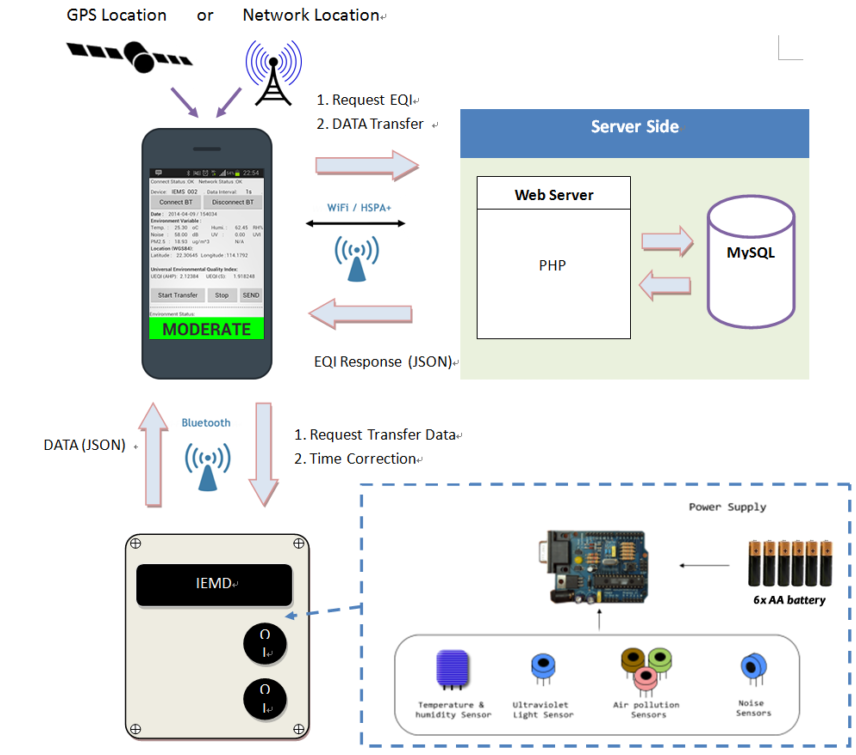
\includegraphics[scale=0.34]{images/fig1.png}
  \hspace*{-1.25cm}
  \caption{System Architecture:IEMD}
  \label{arch}
\end{figure}


\begin{enumerate}
\item	Integrated Environmental Monitoring Device(IEMD).
\item	Handheld Remote Control Panel(RCP).
\item	Web Server.
\end{enumerate}

 
IEMD is portable device which consists of MCU, sensors, wireless communication module. The device is powered using six AA batteries. Sensors used are temperature and humidity, UV, PM, Noise Sensor.
The processor or MCU used in this is Arduino Nano board, and all the sensors are integrated into this MCU and the communication module used here is HC-06 blue tooth module.
RCP is an android application which is an interface for the device control. This does the data exchange between IEMD and Web Server. RCP on receiving information from IEMD, then it will transfer whole data to webserver using Apache HTTP.
Web Server provides a real time data visualization and data analysis. The paper has conducted a field test at several locations for evaluating the functionality of system. It showed that the system worked well. There were two main problems which cited:
\begin{enumerate}
\item GPS positioning accuracy was relatively low.
\item Low battery life.

\end{enumerate}



\section{Air Sense: An intelligent home-based sensing system for indoor air quality analytics}

Air sense is an excellent approach to assess the quality of indoor air. The paper tries to introduce the idea of Indoor Air Quality to the society by proposing a system which measures indoor pollution as the current society is miss-informed or ignorant about it. The system works through electronic sensors which are coupled to a Arduino (processing unit). The system not only extracts the data, but also provides its customers with very effective visualization and analysis of the data. This system has made use of some machine algorithms for the data analysis so as to provide intelligence to the system. The researchers of the paper have done an excellent work on developing this robust system that would sense the pollution and provide education and awareness among the users.
\begin{figure}[h!]
  \centering
  \hspace*{-1.25cm}   
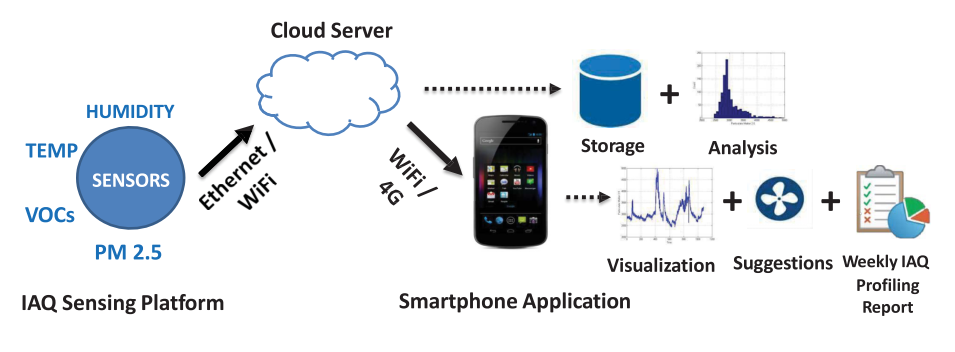
\includegraphics[scale=0.34]{images/fig2.png}
  \hspace*{-1.25cm}
  \caption{System Architecture:Air sense}
  \label{arch}
\end{figure}

The main challenge in the system was to present the extracted data in such a way that, anyone irrespective of their backgrounds could understand the data and importance of Indoor Air Quality. This posed the system three sub challenges which included Pollution Event Detection, Source Identification and IAQ Forecast. All these were to be found from three sensor readings. This paper was able to successfully use some state of the art machine learning algorithms to accurately predict the pollution sources and forecast their behavior. The system has also got a smart phone application which gives the users a very effective interface for visualizations and understanding the data.
The main weakness of the paper is that the pollution sources have been limited to very few. The second weakness is that the prediction has been carried out on historical data rather than the data related to pollution in a particular area or state.
\section{IOT Enabled Proactive Indoor Air Quality Monitoring System for Sustainable Health Management.}
This system measures the indoor air quality. All though the paper discussed about a variety of pollutants and pollution events, the author's interest in office environment wherein the pollution to the gases from electronic devices and machines are high. Hence the system considers Ozone gas to be the primary pollutant. The author has put forward an idea of transmitting data through a Bluetooth channel and process the data in a Wi-Fi Network. The paper also discusses about the new construction design wherein the ventilation is very less which might lead into the presence of numerous sources of synthetic chemicals which has resulted in elevated concentrations of volatile organic compound inside the rooms. One such machine is the photocopiers, which is known to emit poisonous gases like ozone. The system consists of 4 nodes.
Sensing node which is a Arduino which acquires the data from the sensors
Ozone sensor which measures the level of ozone and sent it to the sensing node. 
Gateway node which used to transmit the acquired data through Bluetooth and finally a processing node which process the data.
Overall, the paper only discusses ozone as pollutant in the system neglecting all the other pollutants.

\section{Toward On-Demand Urban Air Quality Monitoring using Public Vehicles.}

The paper discusses an effective method to acquire air quality data in an urban area. In the earlier systems the sensing module was fixed at different stations and therefore will only measure the air quality in the vicinity.


\begin{figure}[h!]
  \centering
  \hspace*{-1.25cm}   
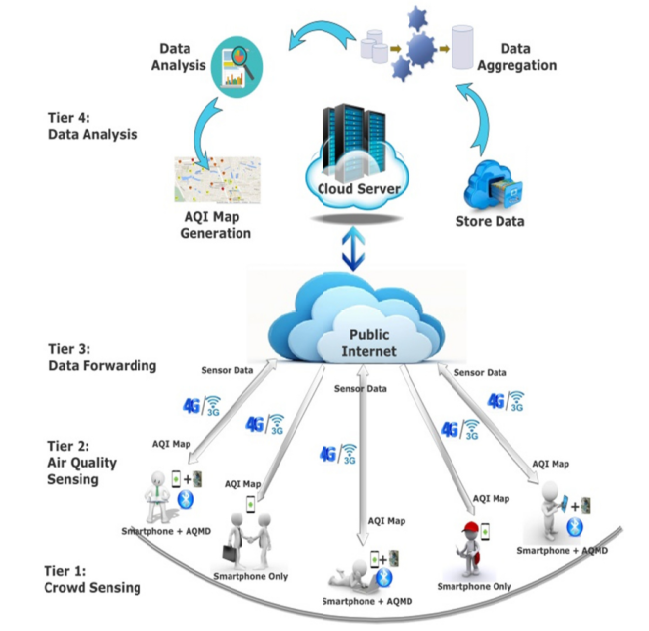
\includegraphics[scale=0.34]{images/fig3.png}
  \hspace*{-1.25cm}
  \caption{System Architecture}
  \label{arch}
\end{figure}


 The system proposed has the sensing unit kept on a public vehicle which keeps on moving in and around the city. The system has made use of garbage trucks and garbage patrol vehicles due to above mentioned reasons.
The paper's main focus is in pollutants like PM, CO and SO. The system is also aided with GPS system so that the sensors values could be mapped onto the locations. To remotely monitor the sensing conditions and to check for maintenance, a control center tool has also been developed. It consists of a map, graph which tracks the route of the vehicles and the sensor data acquired by each vehicle. The next part of the paper is a monitor which was developed along with the system to send the users the collected data. It estimates the amount of pollution inhaled by the user, by the acquiring the user's location from the mobile application and mapping it to the location-sensors value which has been already computed. It also considers the respiratory volume of the user to estimate the pollution inhalation.

The paper proposes an effective and low cost system to understand the air quality in an urban area.

\section{Towards smart city: Sensing Air quality in city based on opportunistic crowd sensing.}

A crowd sensing based air quality monitoring system is designed which aims at collecting and aggregating sensor data for air pollution monitoring in city. An air quality monitoring system(AQMD) was made and connected with smart phones and the information was gathered and shared to cloud. Air sense developed here is a 4 tier architecture consist of crowd which provides data, the dealing with data which means air quality sensing, transferring of data (data forwarding from smart phone to cloud) and finally the data analysis which is storage, aggregation and analysis. Finally, the result computed in tier 4 is sent back to tier 1 through tier 3. The AQMD consists of sensors, a Bluetooth module, Arduino and a power supply. Arduino interfaces between sensor and Bluetooth module. whenever there is a change in air quality Arduino communicates with Bluetooth module and then data are transmitted to smart-phones via Bluetooth. In smart-phone the data from Arduino is collected, transferred to cloud and provide AQI map.

\section{MyPart: Personal, portable, accurate airborne particle counting}

The primary air pollutant for major health issues is small airborne particles of size less than 10 microns and due to which a particle sensor named My-Part was developed which is of low cost. My-part sensor differs from the other sensor available in market in the following features accessibility, flexibility, portability and accuracy.
	 The paper compares My-part to the existing sensor system such as thermal based gas sensors and states that either some system consists of low cost gas sensors which does a poor job of accurately measuring the actual gas concentration due to sensor response selectivity and gas interaction problems with sensor. 
	 Next comparison is done with low cost led and photo diode based sensors and states that these sensors give unreliable readings especially at lower concentration. Another comparison is done with laser and photo diode based sensors and points that these system performs poor in outdoor and there is ambient light leakage. The design of My-Part is based on traditional laser based photo diode system with improvement in airflow to remove light leakage, integration of structural design and circuitry for ambient visualization, BLE transceiver for low power networking and also mobile application for visualization. Two main issues tackled by  is accuracy and calibration of sensor which no existing consumer sensor has addressed. A mobile application was also developed in addition to the hardware.



\chapter{Problem Statement}

The quality of the air we breathe not only impacts individual's health but also has a significant cumulative effect on public health, global environment, and worldwide economy \cite{AQI14}. Air pollution can cause heart disease, chronic obstructive pulmonary disease (COPD), stroke, and lung cancer, etc. On a daily basis, people could suffer from difficulty in breathing, coughing, wheezing, and asthma \cite{AQI14}.My aim is to create a simple pollution monitoring system which would educate the common lay men on the adverse effect of air pollution by showing them how polluted is their vicinity.  This can be done by including all the possible pollutants that degrades the air quality. With the help of open source visualization tool, I aim to display the concentration of each pollutant and a combined measure which would define the quality of the air. This can be taken as the first step towards making a software which can exclusively display the values of pollutants. 
Some important questions to be addressed related to the issue of air quality are: What kind pollutants affect the human health most? How to measure them? Who should participate in the measurement? As the pollution is in the atmosphere, should it not be measured everywhere all the time? If so, what kind of infrastructure is needed to facilitate such a ubiquitous measurement? Pollution is a complex mixer of gases and other pollutants. Simply measuring and displaying individual pollutants may not be useful. What kind of metrics are useful for both the public and decision making authorities? These metrics must educate the public, rather than confuse, to avoid breathing polluted air and also influence the authorities to act to mitigate. Basically, they should help authorities to make suitable policy decisions that could in turn influence the polluters to change their behavior.
The main idea behind this system is that it had to be low cost, energy efficient and small in size and it should measure all the major pollutants. A visualization software can be build which takes in the value from the system through a certain communication communication module and displays the value instantly. Apart from just representing the concentration of each pollutant, there can be certain scales such as Air Quality Health Index(AQHI) or Air quality Index(AQI) whose algorithm can also be implemented and represented in the proposed software. 
By the end of this thesis, I believe that it can contribute towards encouraging and helping citizen science to solve the issue of air pollution and also it can help students or researches who are interested in the same area to build hardware and software efficiently .


\chapter{Solution Strategy}

\chapter{Challenges}

\chapter{Time-Line}

\chapter{Progress}

The hardware part of the system was implemented and the values were collected and represented in an open source platform, Thingspeak, which plotted the value of each pollutant concentration corresponding to a particular time.
\section{Architecture of proposed framework}
As proposed, a higher level generic framework to guide building a air pollution monitoring system using low cost commodity hardware and open source software. As the choices for these hardware and software components are enormous and is keep changing as the technologies advance, suggesting one specific combination is hard and also not helpful if the hardware is not available globally at low cost. Therefore, I decided to experiment with a few options of using most commonly available hardware components. To start with, we designed a functional air pollution monitoring hardware system.
The system shown in has three main hardware components:
\begin{enumerate}
\item  Sensors.
\item  Microcontroller board.
\item  WiFi communication module.
\end{enumerate}

\begin{figure}[h!]
  \centering
  \hspace*{-1.25cm}   
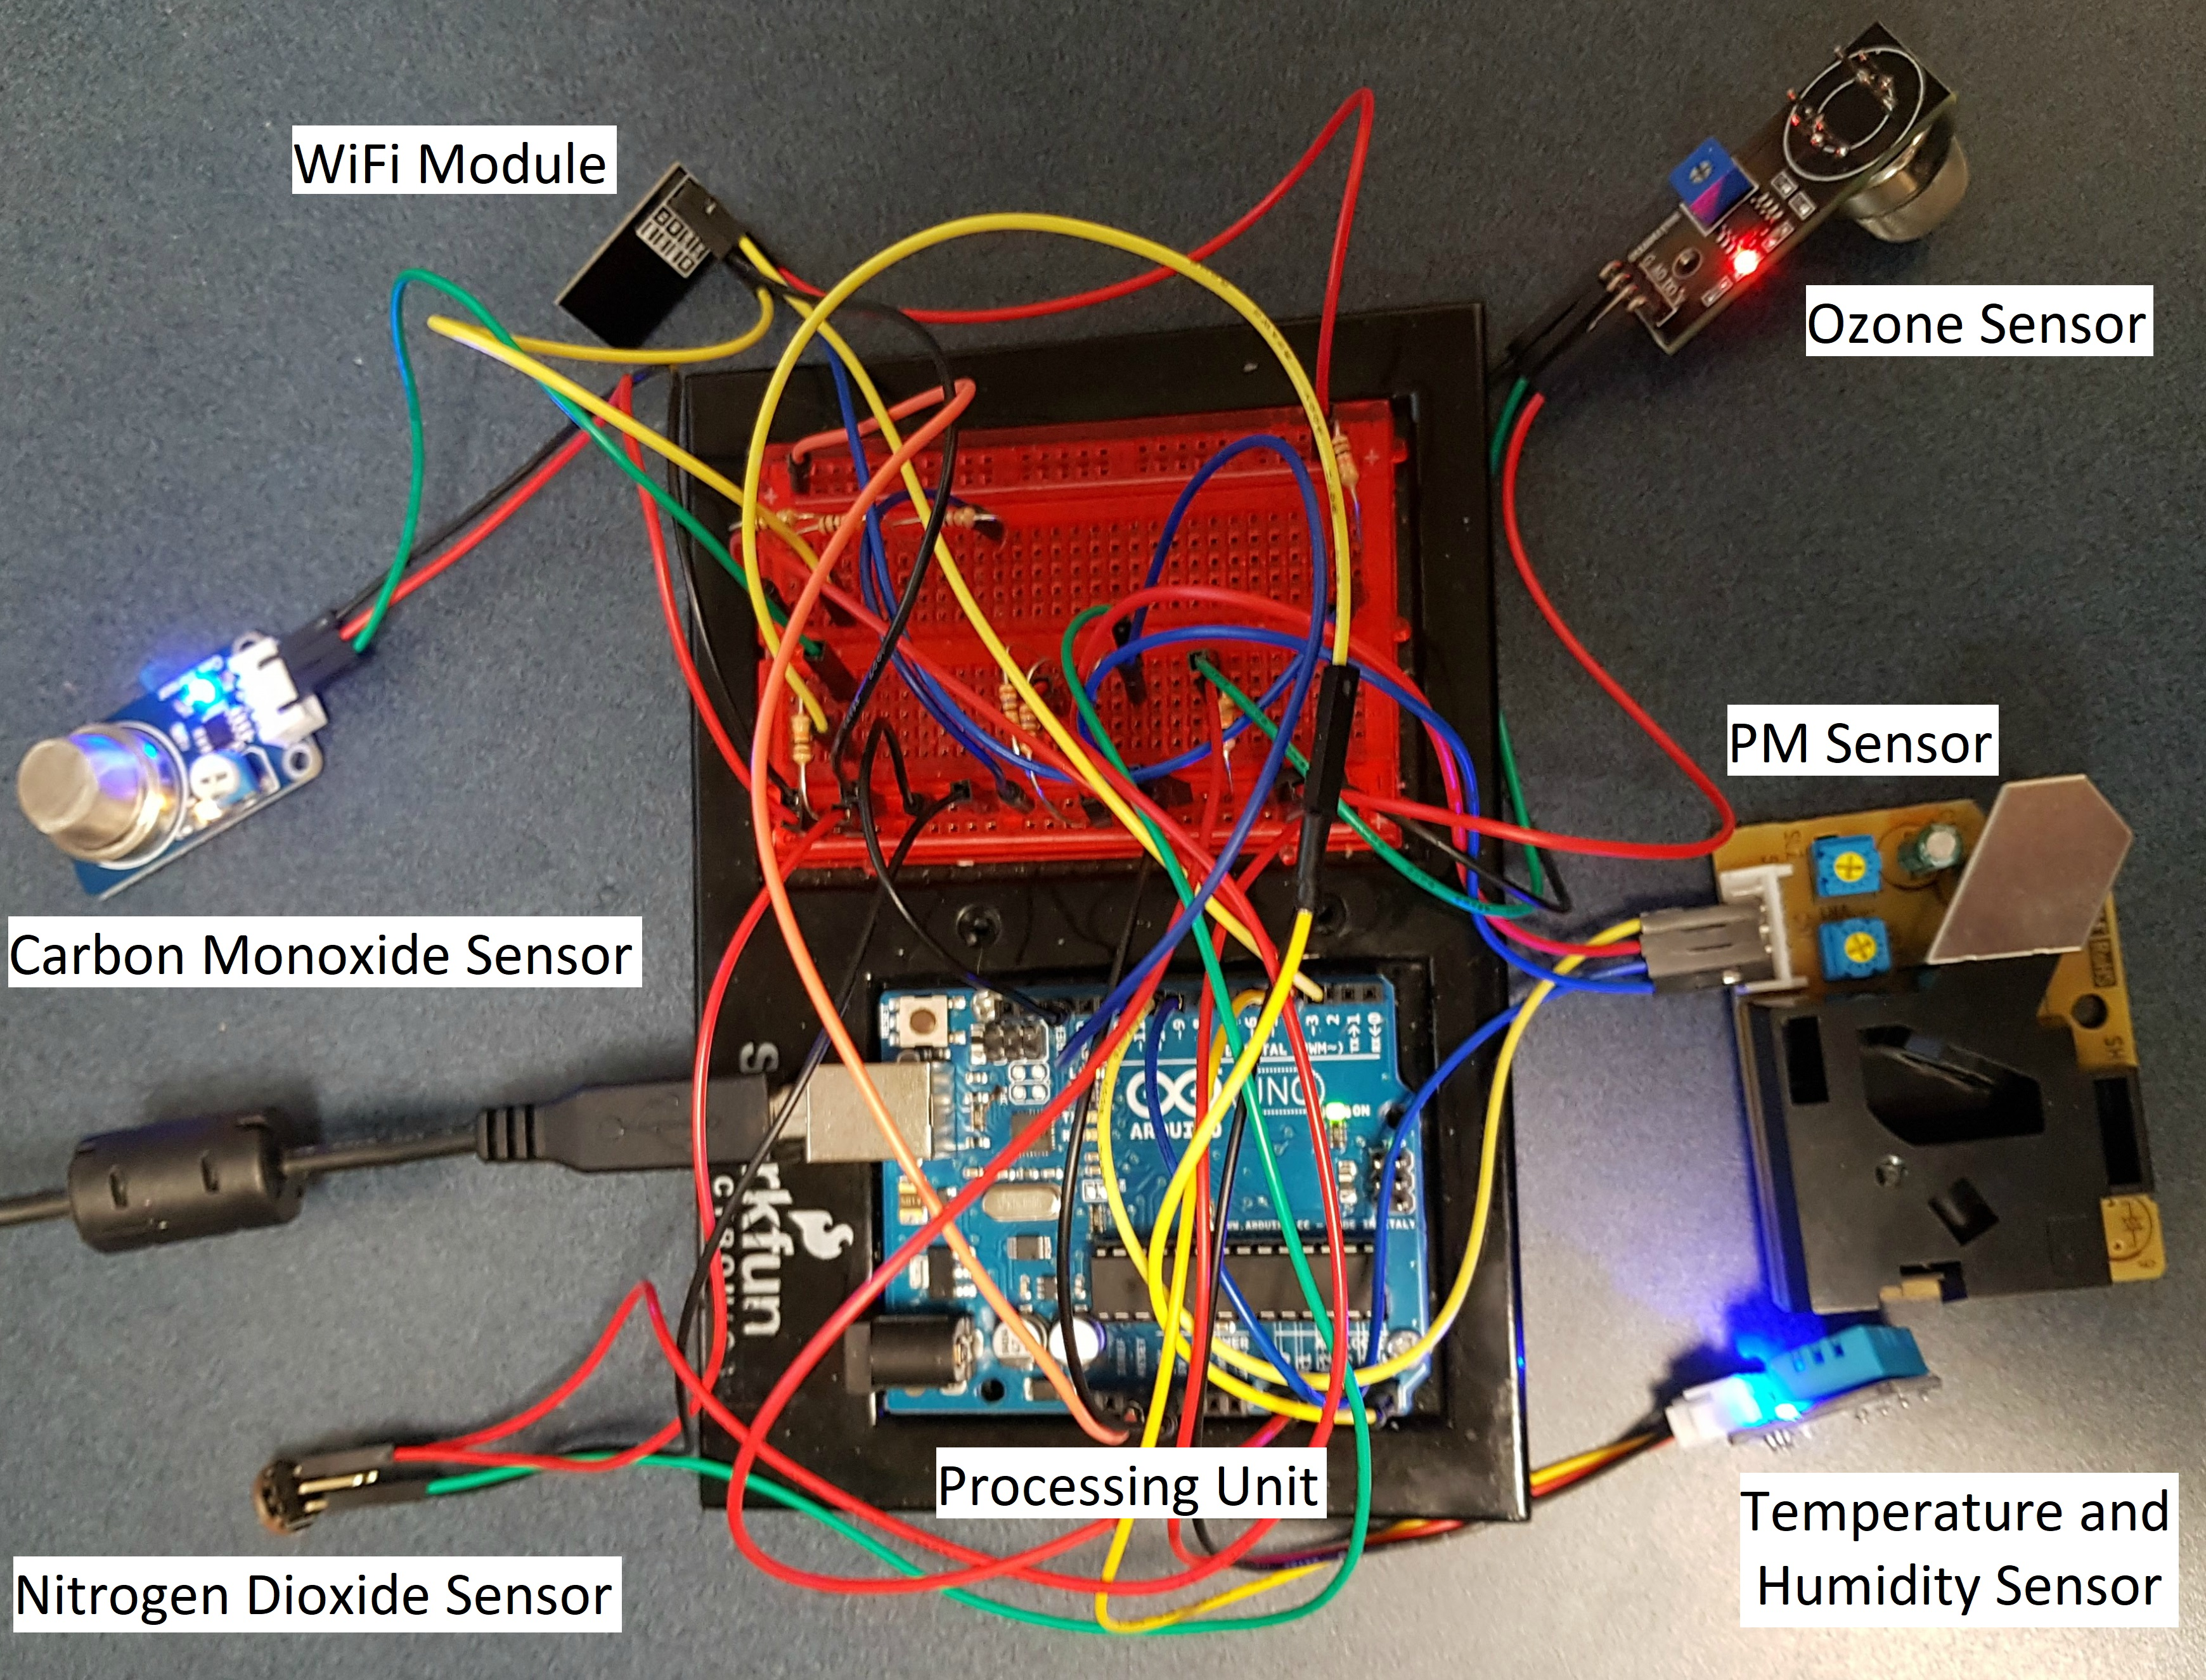
\includegraphics[scale=0.094]{images/fig4.jpg}
  \hspace*{-1.25cm}
  \caption{System Architecture}
  \label{arch}
\end{figure}
\section{Sensors}

Based on the severity of health impact, different countries measure different set of pollutants. For example, India measures 8 major pollutants such as particulate matters (PM), ozone (O3), nitrogen dioxide (NO2), carbon monoxide (CO), sulfur dioxide (SO2), ammonia (NH3), and benzene (C6H6) (in some places lead (Pb) instead). Most other countries measure a subset of these pollutants and, for example, Canada measures PM,O3,NO2,SO2 and CO \cite{HR13}.
 In addition to temperature and humidity sensors, we integrated four sensors into our system to measure four major pollutants such as PM,O3,NO2, and CO. Additional sensors can be easily integrated into our setup. The PM sensor Shinyei PPD42 that we integrated in our system can measure both PM2.5 and PM10. The MQ series sensors MQ-131 and MQ-2, respectively, are used to measure the concentration of O3 and CO in the air. The MICS-2714 sensor is used to measure the concentration of NO2 in the air.
 \section{Microcontroller Board}
 For simplicity and ease of programming, I have use Arduino Uno which internally has ATmega328 microcontroller board. Since it is open-source based platform with rich software support, it is a widely used platform for various applications. Arduino supports both digital and analog inputs. It has 14 digital pins and 6 analog pins, and has shield to connect with both Ethernet and WiFi. As edge computing is preferred in this context, most of the calculation such as measuring gas concentration and computing air quality and air quality health indices are done in Arduino.


 \section{Communication Link}
 For the sensor device to communicate with the IoT software platform for data analytic and visualization services, we use ESP8266 WiFi module that has a networkable microcontroller. This module is very compact and has high durability and power saving features. Once the module is connected to the network it can transfer the data from Arduino to the specified IoT platform by using simple write commands.

\section{Software Platform}
 I have used an open source IoT platform called Thingspeak \cite{Thingspeak}. It is integrated with the system to aggregate, analyze, visualize, and store the sensor data that we collect\cite{Thingspeak}. Thinkspeak can allow many users to integrate their system with other systems for collective and cooperative analysis of sensor data and promote citizen science in solving important global problems. It also offer a ‘hub’ model for data repository and a set of APIs for accessing and using the sensor data for their analysis and interpretations. Thinkspeak provides an intuitive user interface that is easy to understand. It also provides a mobile application called Thingview which can be installed on phone and the same data from the system can be visualized simultaneously.
For this purpose, I have used Thinkspeak to display the results. As soon as the value is transferred to Thingspeak, it can immediately draw graph showing online visualization.In total eight channels of Thingspeak for the graph representation of all the pollutants measured by the sensors and Air Quality Health Index(AQHI).




\chapter{Summary}

\chapter*{References}


\begin{enumerate}

\bibitem{A16} G. Anthes, Open Source Software No Longer Optional, {\it Communications of the ACM}, 59(8):15-17, 2016.

\bibitem{Retal17} M. Rahman, et. al., Adaptive Sensing Using Internet-of-Things with Constrained Communications, {\it ACM/IFIP/USENIX Middleware Conference}, 6 pages, 2017.

\bibitem{Betal17} A. Bagnato, et. al., Designing Swarms of Cyber-Physical Systems: the H2020 CPSwarm Project, 
{\it ACM International Conference on Computing Frontiers}, Invited Paper, 305--312, 2017.

\bibitem{S16} John A. Stankovic, Research Directions for Cyber Physical Systems in Wireless and Mobile Healthcare,
{\it ACM Transactions on Cyber Physical Systems}, 1(1):1:1--12, 2016.

\bibitem{O17} S. F. Ochoa, G. Fortino, and G. D. Fatta, Cyber-physical systems, internet of things and big data (Editorial), {\it Future Generation Computer Systems}, 75:82--84, 2017.

\bibitem{Getal17} G. Guan, et. al., TinyLink: A Holistic System for Rapid Development of IoT Applications,
{\it The 23rd ACM Annual International Conference on Mobile Computing and Networking (MobiCom)}, 2017.

\bibitem {HealthEffectsInstitute2017} Health Effects Institute. State of Global Air 2017. {\it Report}, Health Effects Institute, 2017.

\bibitem{DCRMG17} Joy Dutta, et. al., . Towards Smart City: Sensing Air Quality in City Based on Opportunistic Crowd-sensing. {\it Proceedings of the 18th International Conference on Distributed Computing and Networking}, 42:1--6, 2017. 

\bibitem{YLMLLM15} Wei Ying Yi, et. al., (2015). A Survey of Wireless Sensor Network Based Air Pollution Monitoring Systems. Sensors,  15: , 2015. 

\bibitem{YLL12} James J.Q.Yu, et. al., (2012). Sensor deployment for air pollution monitoring using public transportation system. 2012 {\it IEEE Congress on Evolutionary Computation}, 2:1--7, 2012.  

\bibitem{N15} N. Nannoni,  Message-oriented Middleware for Scalable Data Analytics Architectures.  2015.

\bibitem{KBHG14}
O. Kononenko, O. Baysal, R. Holmes, and M.W. Godfrey. Mining modern repositories with elasticsearch. \textit{In Proceedings of the 11th Working Conference on Mining Software Repositories}. 328-331, May, 2014.

\bibitem{FSK17} M.F.M Firdhous, B.H. Sudantha, P.M. Karunaratne. (2017). IoT enabled proactive indoor air quality monitoring system for sustainable health management. 
{\it Proceedings of the 2nd International Conference on Computing and Communications Technologies (ICCCT)}, 216--221, 2017.

\bibitem{WYM14} Man Sing Wong,Tsan Pong Yip,Esmond Mok,(2014). Development of a Personal Integrated Environmental Monitoring System. {\it Sensors}, 14(11):22065--22081, 2014. 

\bibitem{FXP16} Biyi Fang, et. al.,  AirSense: An intelligent home-based sensing system for indoor air quality analytics. {\it Proceedings of the 2016 ACM International Joint Conference on Pervasive and Ubiquitous Computing}, 109--119, 2016.

\bibitem{H14} Holstius, D. (2014). Monitoring particulate matter with commodity hardware, {\it PhD Thesis}, University of California Berkeley, 2014.

\bibitem{FXPZ16} B.Fang, Q.Xu, T.Park,M.Zhang, (2016). AirSense: An intelligent home-based sensing system for indoor air quality analytics.{\it UbiComp 2016 - Proceedings of the 2016 ACM International Joint Conference on Pervasive and Ubiquitous Computing}

\bibitem {AQI14} Government of India,Ministry of Environment, F.C.C.(2014) National Air Quality Index,58. Retrieved from {\it http:www.indiaenvironmentportal.org.} Air Quality Index.pdf
\bibitem{HR13}  H. Chen,R. Copes,(2013). Review of Air Quality Index and Air Quality Health Index.

\bibitem{Thingspeak} {\it https://thingspeak.com/}



\end{enumerate}

























\end{document}